Una vez introducido el diseño general del sistema, en este capítulo se explicarán los agentes especializados que acceden a las fuentes de datos del proyecto software. 

Para ello primero se introducirá la estructura de la base común \opus{SpecializedAgent}, tras lo que se detallarán tanto las herramientas como el grafo de los cinco agentes especialistas que extienden esta base.

\section{Estructura SpecializedAgent}
El grafo común de este agente se divide en tres pasos generales; la configuración del prompt inicial a utilizar mediante la función \opus{prepare_prompt()} heredada de \opus{BaseAgent}, la ejecución de un subgrafo que implementa el patrón ReAct (Véase Sección \ref{}) y la ejecución de un agente resumidor en caso de ser necesario. La ejecución del grafo general se ilustra en la Figura \ref{fig:specialized}, mientras que el código que lo compone se detalla en el Listado \ref{spec_graph} 


\begin{figure}[h]
  \centering
  \adjustbox{center=\textwidth}{\hspace{-1.2cm}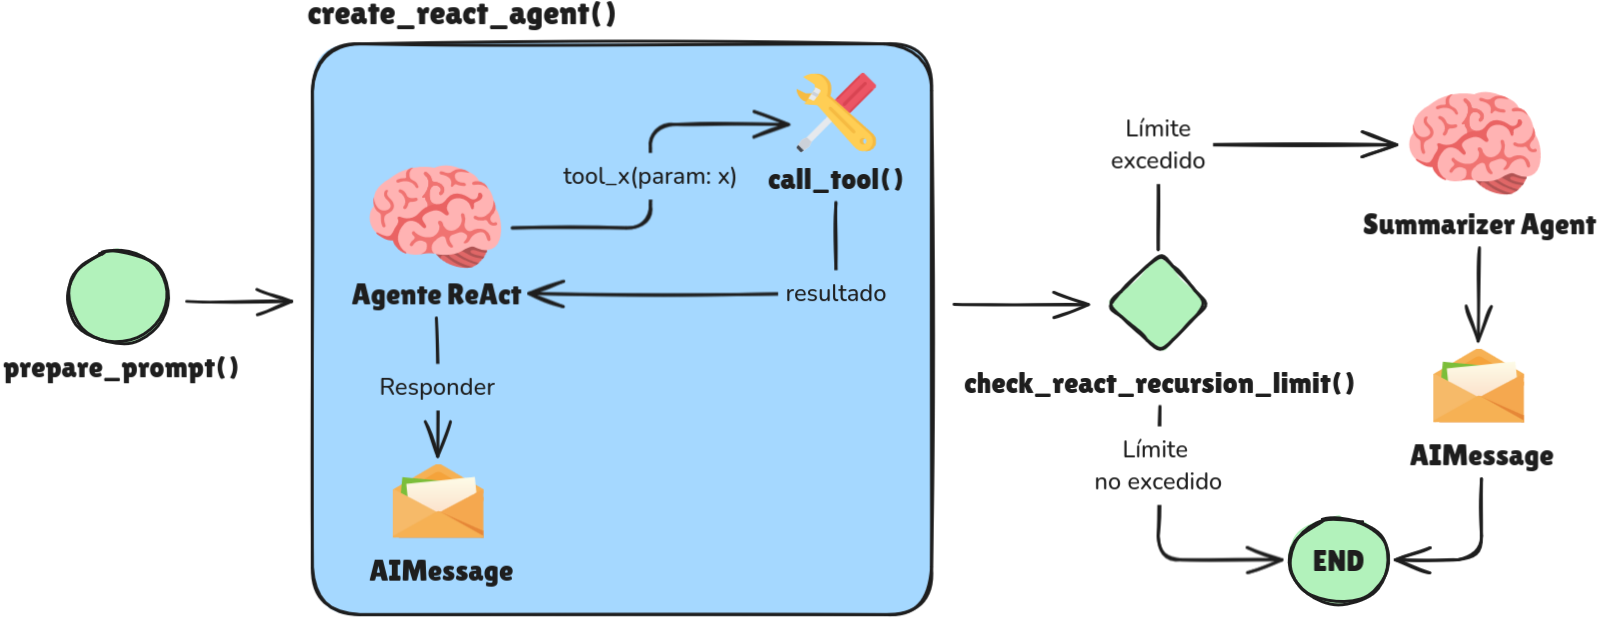
\includegraphics[width=1.3\linewidth]{figures/specialized.png}}
  \caption{Grafo de ejecución de agentes especializados}
  \label{fig:specialized}
\end{figure}

\begin{lstlisting}[caption={\protect\opus{create_graph: Grafo de agentes especializados} },label={lst:spec_graph}]

  def create_graph(self) -> CompiledGraph:
      # Crear grafo ReAct
      agent_tools = self.get_agent_tools()
      self.react_graph = create_react_agent(
          model=self.model,
          tools=agent_tools,
          checkpointer=self.checkpointer
      )

      # Crear grafo del SpecializedAgent
      graph_builder = StateGraph(AgentState)

      # Añadir nodos 
      graph_builder.add_node("prepare", self.prepare_prompt)
      graph_builder.add_node("react", self.call_langgraph_react_graph)
      graph_builder.add_node("response_summarizer", self.generate_summarized_response)

      # Establecer flujo entre nodos 
      graph_builder.set_entry_point("prepare")
      graph_builder.add_edge("prepare", "react")
      graph_builder.add_conditional_edges("react", self.check_react_recursion_limit)

      return graph_builder.compile()
\end{lstlisting}

El grafo ReAct se ha implementado utilizando el agente prefabricado \opus{create_react_agent()} de LangGraph. Este agente acepta una serie de herramientas y un prompt inicial y entra en un bucle de ejecución en el que el agente llama a herramientas y observa su resultado. El grafo finaliza su ejecución cuando el mensaje del agente no contiene llamadas a herramientas, es decir, cuando contiene la respuesta final. 

Se ha establecido un límite de iteraciones que el grafo ReAct puede ejecutar, ya que se ha observado que en ocasiones entra en un bucle de ejecución excesivamente extenso al no encontrar la información requerida. De esta forma, en caso de llegar al límite de iteraciones, un agente resumdidor intenta generar una respuesta con la información disponible observando todas las ejecuciones de las herramientas. 

Para acceder al estado de ejecución del agente ReAct tras finalizar abruptamente su ejecución por el límite de mensajes, se ha utilizado el sistema de autoguardado de LangGraph. Para ello, en la inicialización del agente se crea un objeto \opus{AsyncPostgresSaver}, vinculado tanto a la base de datos PostgreSQL mediante un Pool de conexión asíncrono como al contexto de cierre asíncrono \opus{global_exit_stack}, el cual se establece como autoguardado del grafo ReAct. De esta forma, como se muestra en el Listado \ref{}, se accede a los mensajes del grafo con el identificador previamente configurado. El uso del guardador asíncrono evita problemas de concurrencia al ejecutar varios agentes asíncronos. 

Para crear este agente primero se debe instanciar el agente indicando parámetros como el nombre, su descripción, el modelo a utilizar y el nombre de las herramientas que se quieren utilizar entre otros. Tras esto, se debe llamar a la función \opus{init_agent()}, la cual creará las conexiones MCP necesarias como se ha detallado en la Sección \ref{sec:gestionmcp}. En caso de necesitar herramientas no disponibles en dicho servidor, la función \opus{add_aditional_tools()} gestionará la lógica integración de estas herramientas.   


La ejecución de estos agentes extiende el proceso de la clase común \opus{BaseAgent} explicada en la Sección \ref{sec:baseagent}. De esta forma, inicialmente el proce 

